\resizebox{0.92\columnwidth}{!}{%
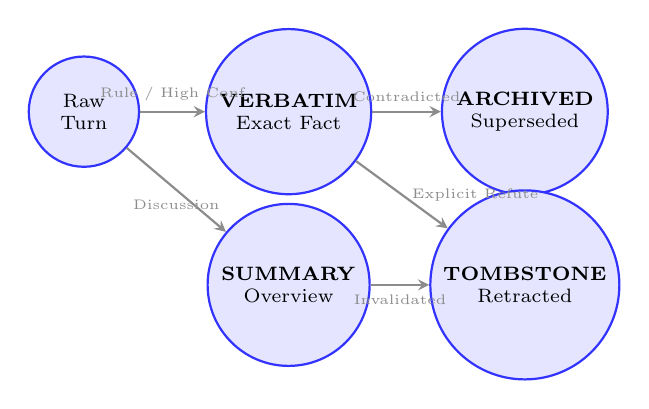
\begin{tikzpicture}[
    state/.style={circle, draw=blue!80, fill=blue!10, thick, minimum size=1.4cm, align=center, font=\scriptsize},
    trans/.style={->, >=stealth, thick, color=gray!90}]

\node[state] (raw) {Raw\\Turn};
\node[state, right of=raw, xshift=1.6cm] (verb) {\textbf{VERBATIM}\\Exact Fact};
\node[state, below of=verb, yshift=-1.2cm] (summ) {\textbf{SUMMARY}\\Overview};
\node[state, right of=verb, xshift=2.0cm] (arch) {\textbf{ARCHIVED}\\Superseded};
\node[state, right of=summ, xshift=2.0cm] (tomb) {\textbf{TOMBSTONE}\\Retracted};

\draw[trans] (raw) -- node[above, font=\tiny]{Rule / High Conf} (verb);
\draw[trans] (raw) -- node[below, font=\tiny]{Discussion} (summ);
\draw[trans] (verb) -- node[above, font=\tiny]{Contradicted} (arch);
\draw[trans] (summ) -- node[below, font=\tiny]{Invalidated} (tomb);
\draw[trans] (verb) -- node[right, font=\tiny]{Explicit Refute} (tomb);

\end{tikzpicture}%
}
